\section{\algo: Deformable-and-Jax Benchmark}
\label{sec:algo}

 \algo\ is a general-purpose differentiable DOM simulation platform that covers a wide range of deformable objects and manipulation tasks. To facilitate benchmarking of DOM methods from all paradigms, particularly differentiable methods, we developed our own differentiable simulator, Deformable-and-JAX (\simulator), which is both highly efficient and parallelizable. In this section, we first provide a brief overview of our simulator, \simulator, and then focus on introducing the benchmark tasks we have implemented for \algo.

\subsection{\simulator}

 \begin{wrapfigure}[12]{r}{0.3\textwidth}
    \centering
    \vspace{-20pt}
    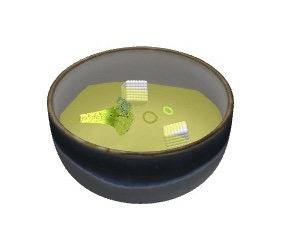
\includegraphics[width=0.7\linewidth]{iclr2023/figs/objects/soup.jpg}
    \captionof{figure}{\small An example of a bowl of soup with tofu and vegetables. All  materials including the soup are simulated by \simulator \space using particles. Moreover, the entire simulation is fully differentiable and highly parallelizable.}
 \label{fig:soup_img}
 \vspace{-10pt}
\end{wrapfigure}

 \simulator\ is a differentiable simulator designed to model various types of deformable object manipulation with high parallelization capabilities. A comparison with other existing simulators can be found in Table \ref{tab:simulator_comparison}. \simulator\ is implemented using JAX \citep{jax2018github}, which supports highly parallelized computation with excellent automatic differentiation directly optimized at the GPU kernel level. Moreover, \simulator\ can be seamlessly integrated with the numerous learning algorithms implemented using JAX, allowing for the entire computation graph to be highly parallelized end-to-end.

\textbf{State Representations and Dynamic Models} \simulator\ adopts different state representations and dynamic systems to model different types of deformable objects with distinct underlying deformation and dynamics. To model liquid and rope, which undergo significant deformation, \simulator\ represents their states using particles and uses Moving Least Square Material Point Method (MLS-MPM)~\citep{hu2018mlsmpmcpic, sulsky1994particle} to model their dynamics on the particle level. For cloth, which only undergoes limited deformation, \simulator\ models its state using mesh and uses a less computationally expensive mass-spring system to model its dynamics. These modeling choices allow \simulator\ to strike a balance between modeling capacity and complexity. For more information on the object models used in \simulator\, please refer to Appendix \secref{sec:object_model}.

\textbf{Designed for Customization} \simulator\ allows full customization of new tasks based on the existing framework. Objects with arbitrary shapes and different rigidness can be added to the simulator with ease. Moreover, primitive actions can also be customized. For a code example of how to customize a new environment in \simulator, please refer to Appendix \secref{sec:code_example}.

\textbf{Saving Memory} \simulator\ uses two tricks to optimize the efficiency and memory consumption of the end-to-end gradient computation, namely lazy dynamic update and ``checkpointing method'' \citep{checkpoint, chen_checkpoint, Griewank_checkpoint}. To optimize the time and memory consumption of MPM for a single timestep, \simulator\ lazily updates the dynamic of a small region affected by the manipulation at that step. Moreover, \simulator\ only stores the values of a few states (i.e., checkpoints) during the forward pass. During the backward propagation, \simulator\ re-computes segments of the forward values starting from every stored state in reverse order sequentially for the overall gradient. For more details on these techniques, please refer to Appendix \secref{sec:saving_memory}.

\subsection{Benchmark Tasks}
\algo\ provides a comprehensive set of Deformable Object Manipulation tasks, including liquid pouring, rope wiping, cloth folding, and sculpting elastoplastic objects, as illustrated in Figure \ref{fig:task}. These tasks are representative of the common deformable objects encountered in daily life.
Additionally, we propose several new challenging long-horizon tasks that require finer-grained control, allowing for better benchmarking of the \emph{scalability} of DOM methods. The horizon of each task is determined by how many steps a human expert takes to finish the task. \algo\ provides a standardized platform for comparing existing methods and future work on DOM. In this section, we provide detailed information on the tasks supported by \algo.

\textbf{Long Horizon Tasks}
The time complexity for the search-based planning method grows exponentially with the planning horizon, known as the ``curse of history''; this is exacerbated by the large state space of deformable objects.
 However, the existing DOM benchmark tasks typically have relatively short horizons. For example, the cloth folding and unfolding tasks in SoftGym consist of only 1-3 steps. \algo\ addresses this limitation by providing tasks with longer horizons, enabling better evaluation of the scalability of search-based planning methods.

\textbf{Tasks without Macro-Actions}
A macro-action can be seen as executing raw actions for multiple steps. 
For example, we can define a \textit{pick-and-place} or \textit{push} macro-action as a 6-dimensional real vector $(x, y, z, x', y', z')$ representing the start $(x, y, z)$ and end $(x', y', z')$ positions of the gripper, and the raw actions are Cartesian velocities of the gripper.
Macro-actions reduce the dimension of the action space and the effective horizon,
and hence make scaling easier for the DOM methods.
However, macro-actions might be too coarse for some tasks.
For example, when whipping a rope to hit a target location, the momentum needs to be adjusted at a relatively high frequency throughout the execution, making macro-actions unsuitable. \algo\ includes tasks that do not have suitable macro-actions to provide a more comprehensive evaluation of DOM methods.

\begin{figure}
\centering
\subcaptionbox{Pour Soup.}{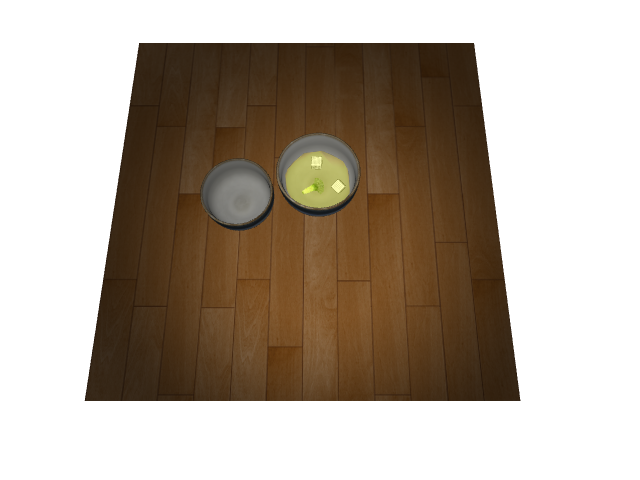
\includegraphics[width=0.19\columnwidth]{iclr2023/figs/tasks/pour_soup_v2.png}}
\subcaptionbox{Push Rope.}{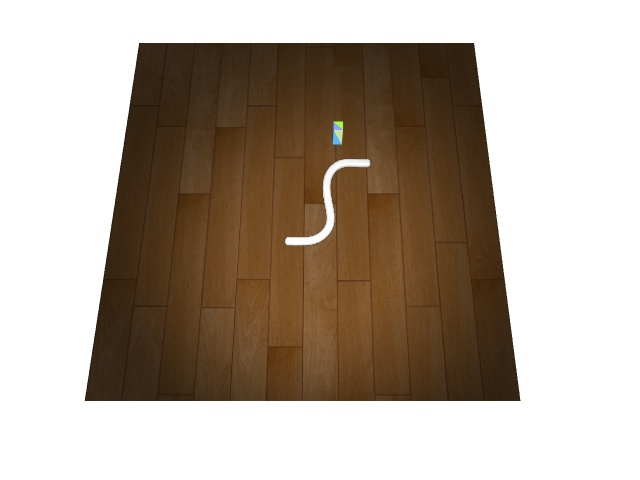
\includegraphics[width=0.19\columnwidth]{iclr2023/figs/tasks/shape_rope_5.jpg}}
\subcaptionbox{Whip Rope.}{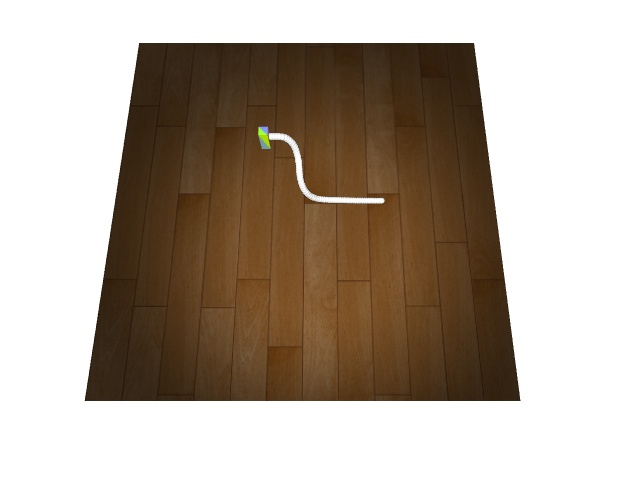
\includegraphics[width=0.19\columnwidth]{iclr2023/figs/tasks/whip_rope_16.jpg}}
\subcaptionbox{Fold T-shirt.}{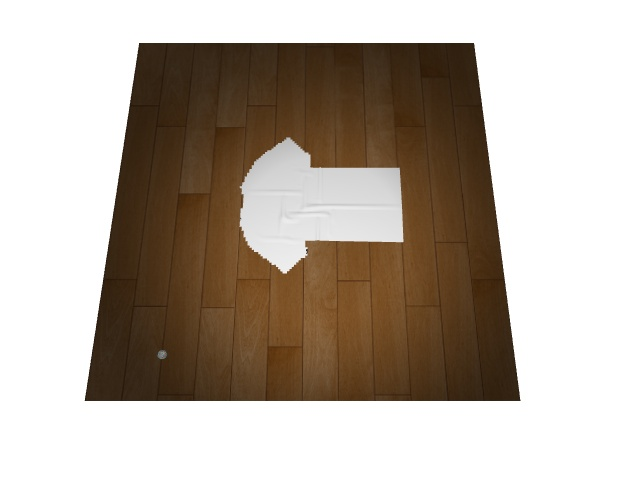
\includegraphics[width=0.19\columnwidth]{iclr2023/figs/tasks/fold_tshirt_0.jpg}}
\subcaptionbox{Unfold Cloth.}{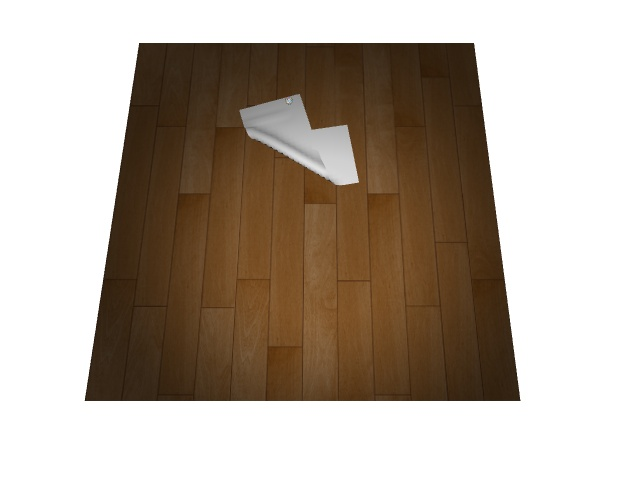
\includegraphics[width=0.19\columnwidth]{iclr2023/figs/tasks/fold_cloth3_6.jpg}}

\caption{
We illustrate different deformable object manipulation tasks in this work. A template is provided to readily expand this set to many other similar tasks. 
  }
\label{fig:task}
\end{figure}
\vspace{-10pt}

\subsubsection{Liquid Manipulation}

\textbf{Pour-Water} Pour a bowl of water into the target bowl as quickly as possible.
The agent directly controls the velocity and rotation (in Cartesian space) of the gripper that holds the bowl. In particular, the action space of the agent is a 4-dimensional vector $a = (v_x, v_y, v_z, w)$, for which $(v_x, v_y, v_z)$ represents the linear velocity of the gripper, and $w$ denotes the angular velocity around the wrist.

\textbf{Pour-Soup} Pour a bowl of soup with various solid ingredients into the target bowl as fast as possible.
The actions are the same as those of Pour-Water.
This task is more challenging than Pour-Water due to the additional interactions between the liquid and the solid ingredients.
In particular, the agent needs to promptly react when a solid ingredient is transferred, so as to 1) adjust for the sudden decrease in load on the gripper and 2) control the momentum of the ingredient when hitting the soup surface to minimize spilling.

Neither tasks have suitable high-level macro-actions and the task horizons are 100 steps.

\subsubsection{Rope Manipulation}

\textbf{Push-Rope} Push the rope to the pre-specified configuration as quickly as possible.
We randomly initialize the configuration of the rope.
The agent uses a single gripper to execute the \textit{push} macro-actions.
The horizon for this task is 6 steps.

\textbf{Whip-Rope} Whip the rope into a target configuration. 
The agent holds one end of the rope and controls the gripper's velocity to whip the rope. In particular, the action space of this task is a 3-dimensional vector $a = (v_x, v_y, v_z)$ that denotes the velocity of the gripper in the Cartesian space.
This task cannot be completed by the abstract macro-actions since the momentum and the deformation of the rope has to be adjusted at a relatively high frequency. The task horizon is 70 steps.

\subsubsection{Cloth Manipulation}

\textbf{Fold-Cloth} Fold a piece of flattened cloth and move it to a target location. This task has two variants: the easy version requires the agent to execute 1 fold and the difficult version 3 folds. For both variants, the task begins with the cloth lying flat on the table at an arbitrary position. The agent executes \textit{pick-and-place} macro-actions. The task horizon is 3 and 4 for the easy and difficult versions respectively.

\textbf{Fold-T-shirt} Fold a T-shirt to a target location. The task begins with the T-shirt lying flat on the table at an arbitrary position. The agent executes \textit{pick-and-place} macro-actions. The task horizon is 4.

\textbf{Unfold-Cloth} Flatten a piece of folded cloth to a target location as fast as possible. This task also has two variants that differ in the initial configurations of the folded cloth: the cloth in the easy version has been folded once and that in the difficult version has been folded three times.
This task has the same action space as the Fold-Cloth task. The task horizon is 10 steps for both variants.

All of these tasks share similar APIs to the OpenAI Gym's standard environments. We provide a general template to define tasks in our simulator. This not only better organizes the existing task environments but also allows the users to customize the existing task environments to better suit their research requirements. The variables and constants defined in the template are easily interpretable quantities that correspond to real physical semantics. This allows the users to better understand the environment, which can also help with the development and debugging process. 


 
 
